\documentclass[12pt, letterpaper]{../assignment}
\usepackage{graphicx}
\usepackage{courier}
\usepackage{minted}
\usepackage{amsmath}
\usepackage{commath}
\usepackage{amssymb}
\usepackage{amsfonts} 
\usepackage{cancel}
\usepackage{enumitem}
\usepackage{array}

\usepackage{tikz}
\usetikzlibrary{shapes,arrows,positioning}

\usemintedstyle{monokai}
\oddsidemargin = 0pt
\exercisesheet{Module 12}{Practice Assignment}
\student{Austin Barrilleaux}
\courselabel{EN 525.609}
\semester{Fall 2023}
\usepackage[backend=bibtex,style=numeric,sorting=none]{biblatex}
\bibliography{reference}
\usepackage{color}
\definecolor{light-gray}{rgb}{0.2,0.2,0.2}
\setminted{bgcolor=light-gray}
\setlength{\parindent}{0pt}

\makeatletter
\patchcmd{\minted@colorbg}{\noindent}{\medskip\noindent}{}{}
\apptocmd{\endminted@colorbg}{\par\medskip}{}{}
\makeatother

\begin{document}
\subsection*{Problem 1}

\subsubsection*{Solve the following 9th Edition textbook problems:\\
\begin{itemize}
    \item 9-49 (a)
    \item 9-50 (c,d)
\end{itemize}}

\subsubsection*{(9-49) Consider that the controller in the liquid-level control system shown in Fig. 9P-10 is a single-stage phase-lag controller:}

$$ \mathbf{ G_c(s) = \frac{1 + a T s}{1 + T s}, \ \ \ a < 1 } $$

$$ \mathbf{ G_p(s) = \frac{10 N}{s(s +1)(s + 10)} } $$

\subsubsection*{(a) For $\mathbf{N = 20}$,
select the values of a and T so that the two complex roots of the characteristic equation correspond to a relative damping ratio of approximately 0.707.
Plot the unit-step response of the output $\mathbf{y(t)}$.
Find the attributes of the unit-step response.
Plot the Bode plot of $\mathbf{G_c(s)G_p(s)}$ and determine the phase margin of the designed system.}

This makes the process:

$$ G_p(s) = \frac{200}{s(s +1)(s + 10)}  $$

The compensated system is:

$$ G_c(s)G_p(s) = \frac{200(1 + a T s)}{s(s +1)(s + 10)(1 + T s)} $$

Rewriting the uncompensated process as:

$$ G_p(s) = \frac{K}{s(s +1)(s + 10)}  $$

$K_\text{SSE}$ to satisfy the SSE requirement is $K_\text{SSE} = 200$.
\\\\
Looking at the root locus of the uncompensated system where $K = 1$,
we can that $K_\text{\%OS}$ for a damping ratio of 0.707 is $K_\text{\%OS} = 4.54$:

\begin{figure}[H]
    \centering
    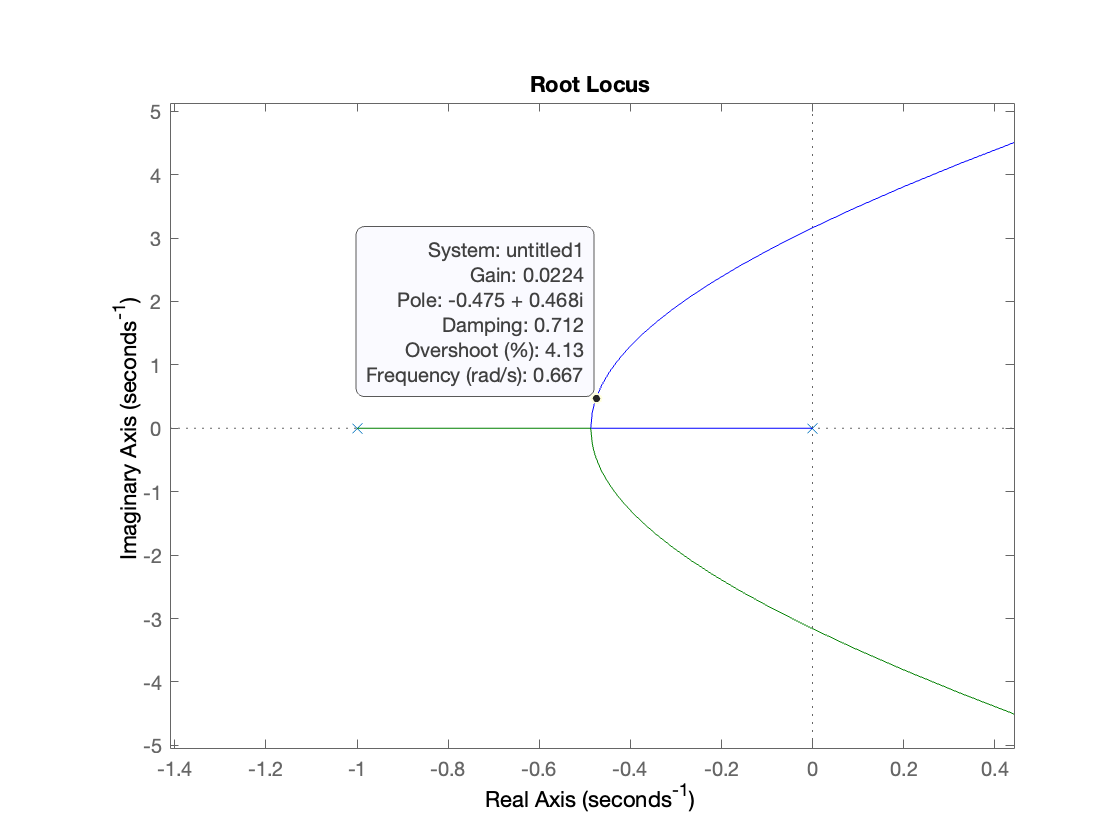
\includegraphics[width=1\linewidth]{./figures/rlocus_9_49a.png}
    % \caption{Root Locus}
\end{figure}

We can calculate $a$ for the compensated system as:

$$ a = \frac{K_\text{\%OS}}{K_\text{SSE}} = \frac{4.54}{200} = 0.0227 $$

If the value of T is sufficiently large, when K =1,
the dominant roots of the characteristic equation will correspond to a damping ratio of approximately 0.707.
Let us arbitrarily select T = 10,000.

% Which can also be written as:

% $$ G_c(s)G_p(s) = \frac{200a(s+\frac{1}{a T})}{s(s +1)(s + 10)(s+\frac{1}{T})} $$

% Looking at a zoomed in view of the root locus plot for the uncompensated system made using the \texttt{rlocus()} function in MATLAB,
% we can see what the complex conjugate roots look like when the damping ratio is roughly equal to $\cos(45^\circ) \approx 0707$:

% \begin{figure}[H]
%     \centering
%     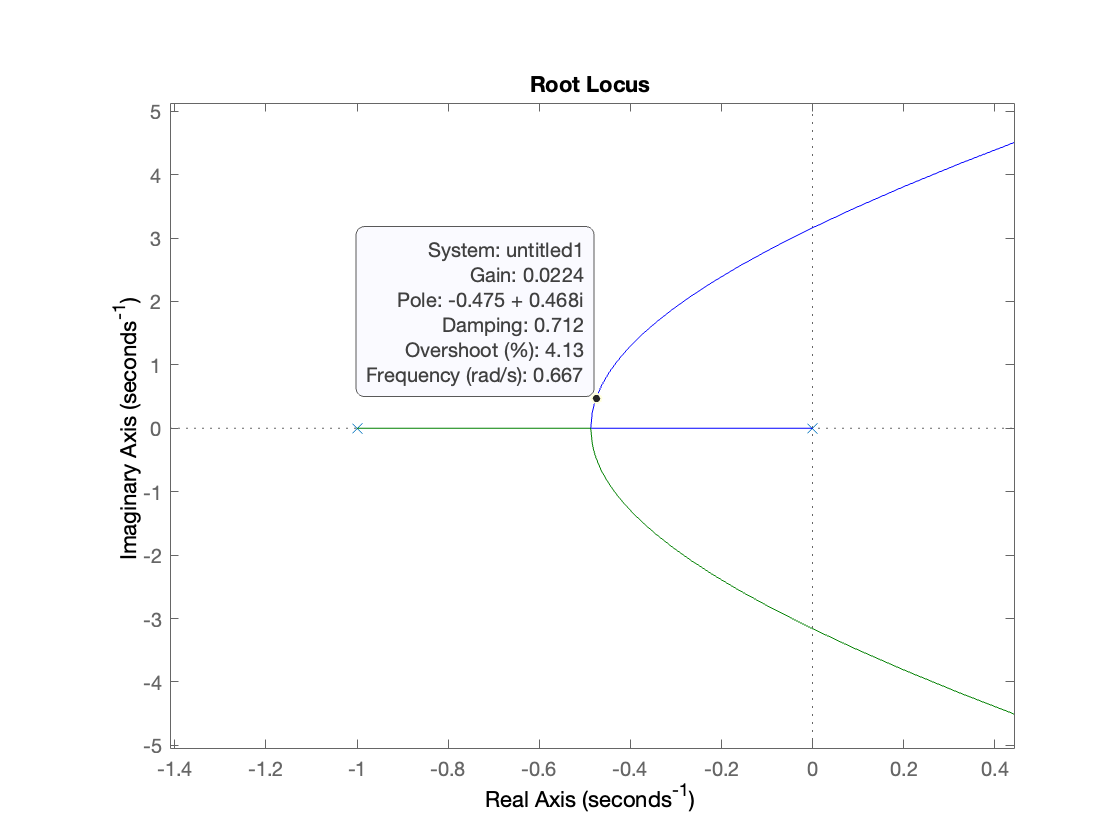
\includegraphics[width=0.7\linewidth]{./figures/rlocus_9_49a.png}
%     \caption{Root Locus}
% \end{figure}

% If we make the assumption that $ \frac{1}{a T} = \frac{1}{T} $, we can write $G(s)$ as:

% $$ G_c(s)G_p(s) = \frac{200a}{s(s +1)(s + 10)} $$

% Using this equation we can solve for $a$ using the following MATLAB code:

% \color{white}
% \hspace*{6em}\inputminted[frame=leftline,fontsize=\footnotesize,
% firstline=8,lastline=29]{matlab}
% {./matlab/P9_49.m}
% \color{black}

% Not that the above algorithm only works given good initial boundaries.

% This solves for a value for $a$ of $a = 0.02268$, where $\zeta - \cos(45^\circ) = -2.22 \cdot 10^{-16}.
% $

% \color{white}
% \hspace*{6em}\inputminted[frame=leftline,fontsize=\footnotesize]{matlab}
% {./matlab/Problem_5_18.m}
% \color{black}

% \begin{figure}[H]
%     \centering
%     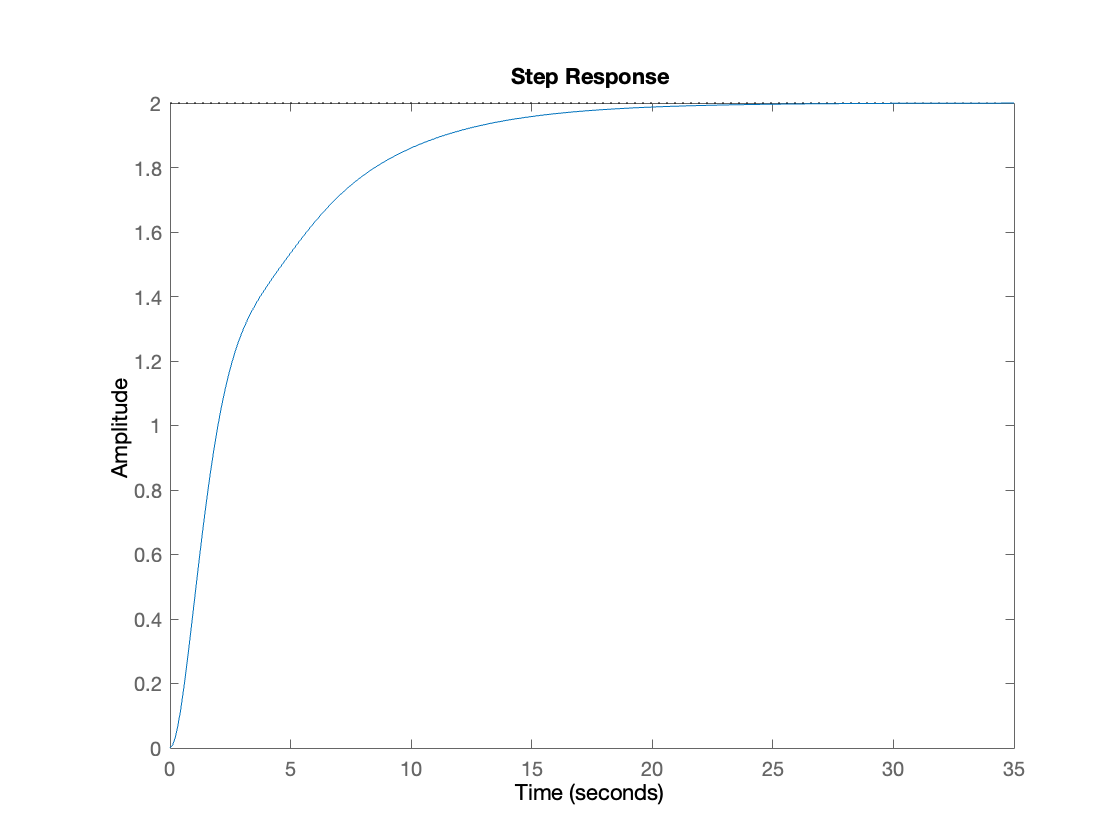
\includegraphics[width=0.7\linewidth]{./figures/step_response.png}
%     \caption{Step Response}
%     \label{fig:step}
%  \end{figure}



\end{document}

